

\section{Introduction}


Video inpainting aims to recover the missing content of a corrupted video and assists lots of practical applications,~\emph{e.g.,} video restoration and watermarking removal. 
High-quality video inpainting requires not only realistic structures with visual details but also temporal consistency. 
%Compared with image inpainting, video inpainting is significantly more challenging due to the extra time dimension, while human eyes are sensitive to flickers and jitters.
% 
Though great progress has been made in 2D image inpainting using deep learning techniques \cite{yu2018free,Xiong_2019_CVPR,wang2018high}, directly applying these approaches to each frame individually for video inpainting will lead to flaws, flickers, and jitters due to the additional time dimension. 





Traditional video inpainting methods employ a patch composition framework that composites visually pleasing content in the missing regions via patches by exploiting complementary information across neighboring frames~\cite{patwardhan2007video,wexler2004space,tcsvt2009,newson2014video}.
% 
These methods rely heavily on the hypothesis that the missing content in the corrupted region appears in neighboring frames, which greatly limits their generalization ability.
%
Recently, deep-learning-based methods achieve great performance improvement in video inpainting \cite{wang2019video,Kim_2019_CVPR1,Xu_2019_CVPR,Kim_2019_CVPR}.
A straightforward solution is to utilize 3D convolution layers to extract spatio-temporal features and predict missing contents with smooth motion \cite{wang2019video}.
To obtain temporally smooth results, contextual information from neighboring frames is aggregated to synthesize corrupted regions using a recurrent feedback scheme~\cite{Kim_2019_CVPR1,Kim_2019_CVPR}, or pixel propagation guided by completed flows~\cite{Xu_2019_CVPR}. 
%For example, a deep optical flow completion network is proposed to propagate missing pixels across frames~\cite{Xu_2019_CVPR}. 
%Kim~\emph{et al.} leverage recurrent feedback to utilize potential information in previous frames~\cite{Kim_2019_CVPR,Kim_2019_CVPR1}.
By integrating motion guidance, these methods pay more attention to temporal smoothness; however, structure rationality and object details have not been well recovered. 


Without definite representation and generation of the target image structures, these methods tend to produce over-smoothed regions. 
Similar observations have been obtained in the image inpainting task \cite{Xiong_2019_CVPR,nazeri2019edgeconnect}.
%\cite{iizuka2017globally,liu2018partialinpainting,yu2018free}. 
To solve this problem, two-step methods are proposed to complete object contours~\cite{Xiong_2019_CVPR} or edge maps~\cite{nazeri2019edgeconnect} first as auxiliary information to guide texture synthesis later in image inpainting.
%
However, when applying these edge-first image inpainting methods to video inpainting, it brings another challenge in generating temporally coherent structures while human vision is significantly sensitive to temporal discontinuity that frequently occurs at edges. 


In order to simultaneously hallucinate detailed image structures and preserve temporal coherence in video inpainting, we present a novel structure-guided video inpainting approach which effectively exploits the spatio-temporal structure information to improve the quality of video inpainting.  
%
Compared with previous video inpainting methods that only consider motion guidance, we explore the correlation between structure, texture, and motion to complete the missing region with reasonable structure, rich visual details, and temporal coherence, as shown in Fig.~\ref{fig:overview}.
% first, edge -- structure
First, we design an edge inpainting network (ENet) to predict sparse edges in the missing region to represent the target structure for each frame by exploiting the spatio-temporal neighboring information from adjacent frames.
%Second, texture
Then, under the guidance of completed edges, we employ a texture inpainting network (TexNet) to fill the missing region via a coarse-to-fine architecture and a structure attention module (SAM).
Specifically, the SAM is designed to guide the texture generation by capturing the latent spatial relevance between video textures and the completed structural edges.
Notably, such a structure-texture relevance can effectively improve the inpainting quality in TexNet with fewer cracks and more realistic object contours.
%Then we fill textures under the guidance of concise edges.
%Third, motion
Furthermore, to enhance the temporal coherence of synthesized frames, we employ motion flows for consistency check of both edge maps and inpainted frames during the training stage.
%
The ground truth optical flow is exploited to guide both ENet and TexNet to generate temporal smooth edge maps and texture results via edge consistency and frame warping losses.%,~\emph{i.e.,} the flow-guided edge warping loss and frame warping loss.
% are respectively utilized to align the edge maps and final inpainted texture between frames. 
Consequently, the inpainted frames using our approach are not only temporally consistent, but also more complete in structure and rich in visual details.

%The detailed comparison between the proposed method and related state-of-the-art methods is given in Table~\ref{tab:comparison}.



%\begin{table}[t]
%\begin{center}
%\caption{Detailed comparison between our method and related state-of-the-art methods. Our method utilizes both auxiliary temporal optimization (Flow) and spatial optimization (Edge), which guarantees spatio-temporal coherence explicitly.} \label{tab:comparison}
%\resizebox{1\columnwidth}{!}{
%\begin{tabular}{c|c|c|c}
 % \hline
  %\multirow{2}{*}{}&Temporal&Spatial&Explicit Spatio-Temporal\\
 % &Opt.&Opt.& Coherence\\
 % \hline
 % \hline
 %Edge-Connect \cite{nazeri2019edgeconnect} &\xmark &Edge& \xmark    \\
 % \hline
 % CombCN \cite{wang2019video} & \xmark &\xmark &\xmark     \\
 % \hline
%  DVI \cite{Kim_2019_CVPR1} &  Flow    &\xmark & \xmark    \\
%  \hline
 % DFVI \cite{Xu_2019_CVPR} & Flow    &\xmark &\xmark               \\
 % \hline
 % Ours&Flow&Edge&\cmark\\
 % \hline
%\end{tabular}%}
%\end{center}
%\vspace{-0.4cm}
%\end{table}


%As shown in Fig.~\ref{zong}, our method mainly consists of two modules, which are respectively an edge inpainting network (ENet) and a texture inpainting network (TexNet).
% and flow guidance constraints (denoted by dotted lines).
%Given multiple adjacent frames with masks, ENet first completes edge maps that depict the target structure via a 3D+2D architecture. 



%In summary, we present a novel structure-guided video inpainting method, which can generate structural reasonable and temporal coherent inpainted frames.
%
We conduct a series of experiments on the YouTubeVOS and DAVIS datasets under different mask settings. 
The results show that the proposed method obtains new state-of-the-art inpainting performance both quantitatively and qualitatively. 
%
Because of the sparsity of edge maps, the computational cost is also greatly reduced.
%
In summary, our technical contributions are three-fold:
\begin{itemize}
	\item We propose a novel structure-guided video inpainting method which integrates scene structure, texture, and motion to complete the missing region with realistic structure, rich visual details, and temporal coherence.
	% explore the correlation 	
	\item A structure attention module is designed to capture the correlation between hallucinated edges and video textures, which can provide better structural guidance for texture synthesis. % edge - texture 
	\item Flow-guided edge and frame consistency constraints are developed to enhance the temporal coherence of the completed edges and video frames.   
\end{itemize}


%The rest of this paper is organized as follows. Section~\ref{sec:rw} reviews the related works. Section~\ref{sec:approach} illustrates the proposed video inpainting method. Section~\ref{sec:exp} provides the experiments on YouTubeVOS and DAVIS datasets, and Section~\ref{sec:conclu} concludes the whole paper.


\begin{figure}[t]
	\centering
	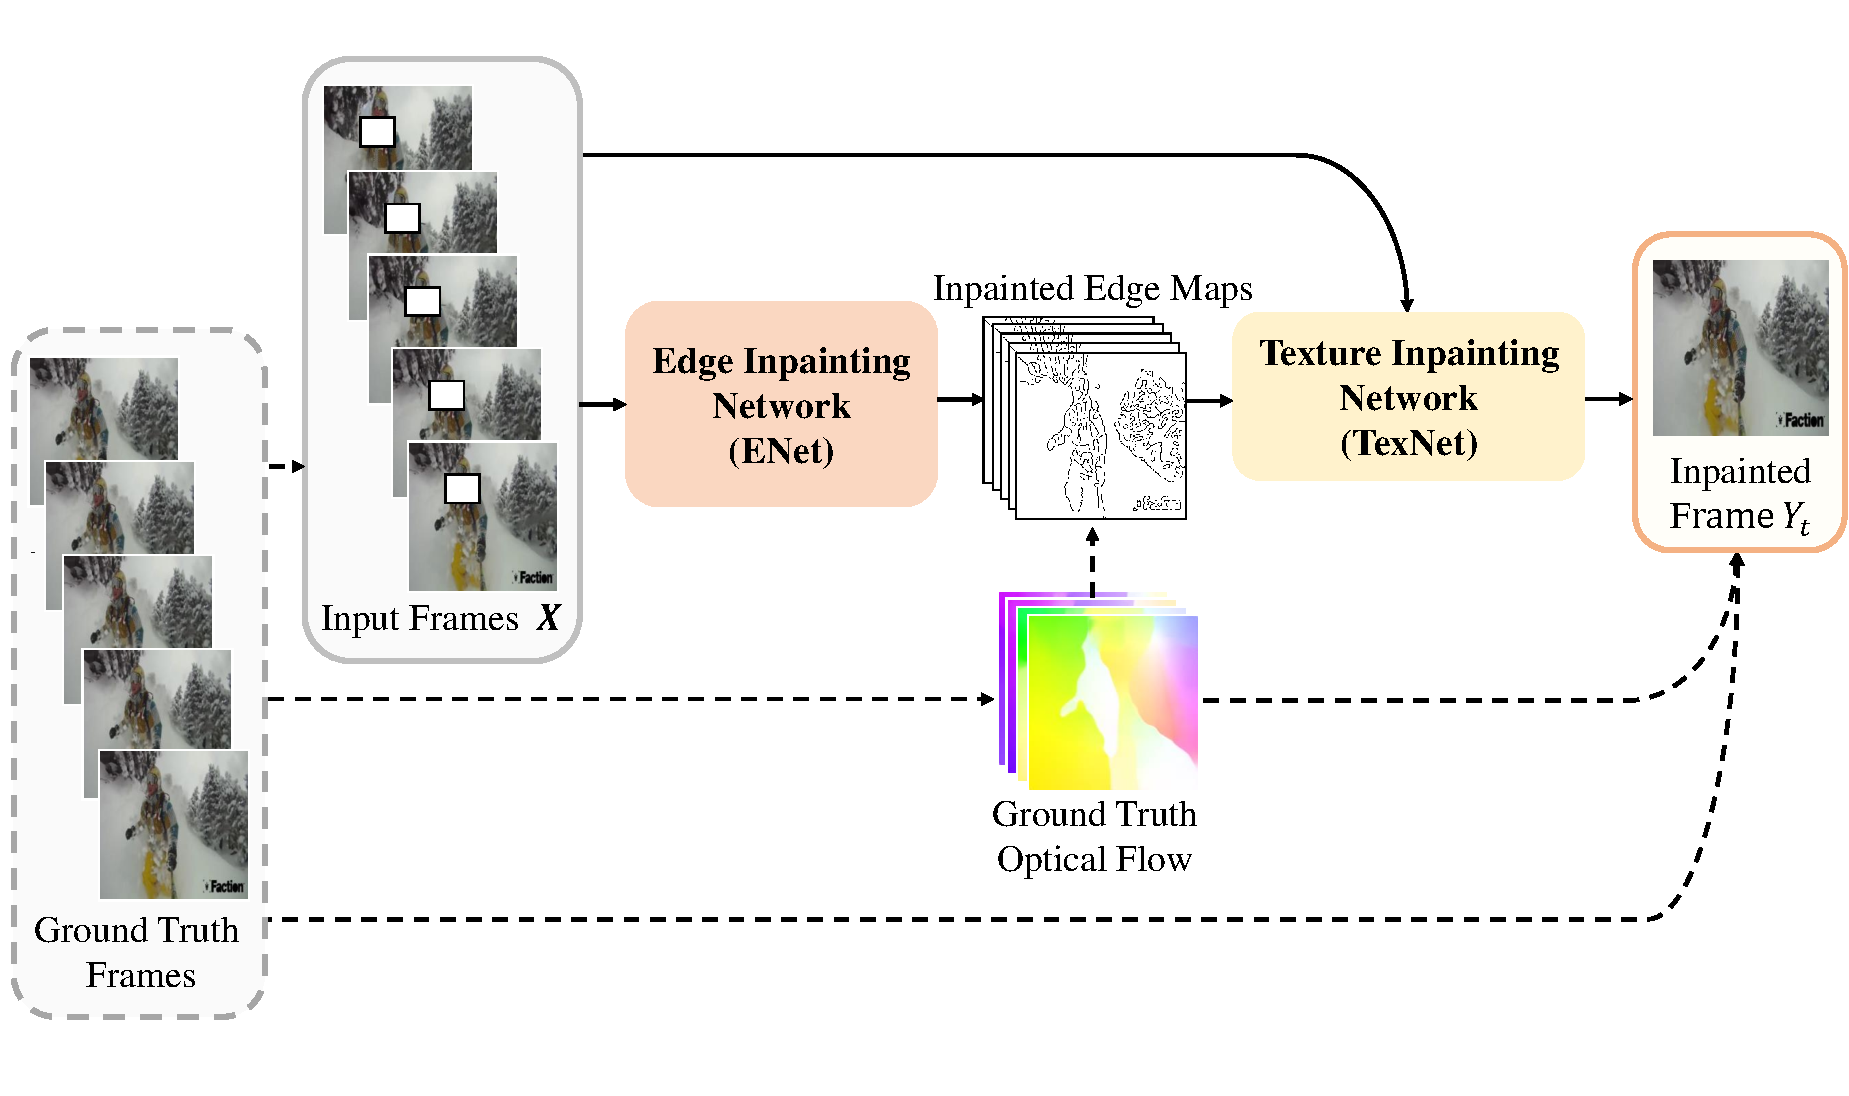
\includegraphics[width=1.01\columnwidth]{zong} % Reduce the figure size so that it is slightly narrower than the column. Don't use precise values for figure width.This setup will avoid overfull boxes. 
	\caption{Overview of our structure-guided video inpainting network. We first complete the missing edges by aggregating information from neighboring frames to represent the target structure using the ENet. Then, the TexNet synthesizes missing textures under the guidance of structure edges. Besides, the ground truth optical flow between frames is utilized during the training stage for both ENet and TexNet to enforce temporal coherence of completed contents, as illustrated by dotted lines.}
	\label{fig:overview}
\end{figure}






\section{Related Work}
%Our method are mostly related to (a) traditional image/video inpainting, (b) CNN-based image inpainting, and (c) deep video inpainting. We will introduce them in this section below.
\paragraph{Traditional Image/Video Inpainting} Image or video inpainting has been studied for decades. 
%
Traditional methods of image and video inpainting can be divided into two categories, diffusion-based and patch-based methods. 
Diffusion-based methods \cite{bertalmio2000image,ballester2001filling,sridevi2019image} gradually propagate contents from surrounding areas to the missing region. 
%
% summary these methods 
%Li \emph{et al.}~\cite{li2016image} define diffusion coefficients according to the relation between the damaged pixels and neighborhood pixels.
%Li \emph{et al.}~\cite{li2017localization} attempt to solve the problem of localization of diffusion-based inpainted regions.
%Fractional-order nonlinear diffusion driven by difference curvature is proposed to produce clearer image details \cite{sridevi2019image}. 
However, this kind of method fails to handle large holes due to its assumption of local smoothness. 
%
Patch-based image inpainting methods, also called exemplar-based methods~\cite{bertalmio2003simultaneous,efros2001image}, are more widely studied.
They formulate the completion task as a patch-based optimization problem. 
Barnes \emph{et al.}~\cite{barnes2009patchmatch} employ approximate nearest neighbor algorithm to fill the damaged regions.
Sangeetha \emph{et al.}~\cite{sangeetha2011combined} propose to propagate both linear structure and two-dimensional texture into the target region.
Ru{\v{z}}i{\'c} \emph{et al.} \cite{ruvzic2014context} introduce Markov random field to search the most matched candidates.
Ding \emph{et al.} \cite{ding_19nonlocal} employ nonlocal texture similarity and local intensity smoothness to produce natural-looking results.
Besides, some patch-based methods utilize low rank approximation. For example, Guo \emph{et al.} \cite{pb_lowrank2018} propose a simple two-stage low rank approximation to recover the corrupted region, which avoids time-consuming iterations.
Lu \emph{et al.} \cite{lu2018gradient} adopt gradient-based low rank approximation.
These patch-based methods fill the missing content by borrowing and aggregating the most similar patches based on low-level image features from known regions. However, they usually fail when there is insufficient information in known regions or image textures are too complicated.  
%

\paragraph{Patch-Based Video Inpainting} Patch-based methods are also widely studied for video inpainting. 
They search similar patches and borrow appearances from known regions across neighboring frames to synthesize the unknown content. 
Wexler \emph{et al.} \cite{wexler2007space} constrain masked regions to synthesize coherent structures with respect to reference examples based on local structures. 
Umeda \emph{et al.} \cite{umeda2012removal} propose using directional median filter as complementation of patch-based filling.
Newson \emph{et al.} \cite{newson2014video} extend the 2D PatchMatch algorithm~\cite{barnes2009patchmatch} into 3D version to improve video inpainting quality.
Huang \emph{et al.} \cite{huang2016temporally} jointly estimate optical flow and textures to promote temporal coherence.
%
Another group of methods separate foreground and background apart, and then deal with the two parts respectively with different algorithms, since there naturally exists property differences between them.  
Ghanbari \emph{et al.} \cite{ghanbari2011contour} first separate the two parts in videos, and fills the two parts accordingly with the help of contours.
Xia \emph{et al.} \cite{xia2011exemplar} make use of Gaussian mixture models to also distinguish moving foreground and still background, and process them separately.   
%However, traditional metshods assume that there exist similar contents in known regions, thus fail to synthesize unseen appearances. 
However, in these patch-based video inpainting methods, the patch-searching process suffers from high computational complexity, thus limiting their usage in practical applications.



\begin{figure*}[!t]
	\centering
	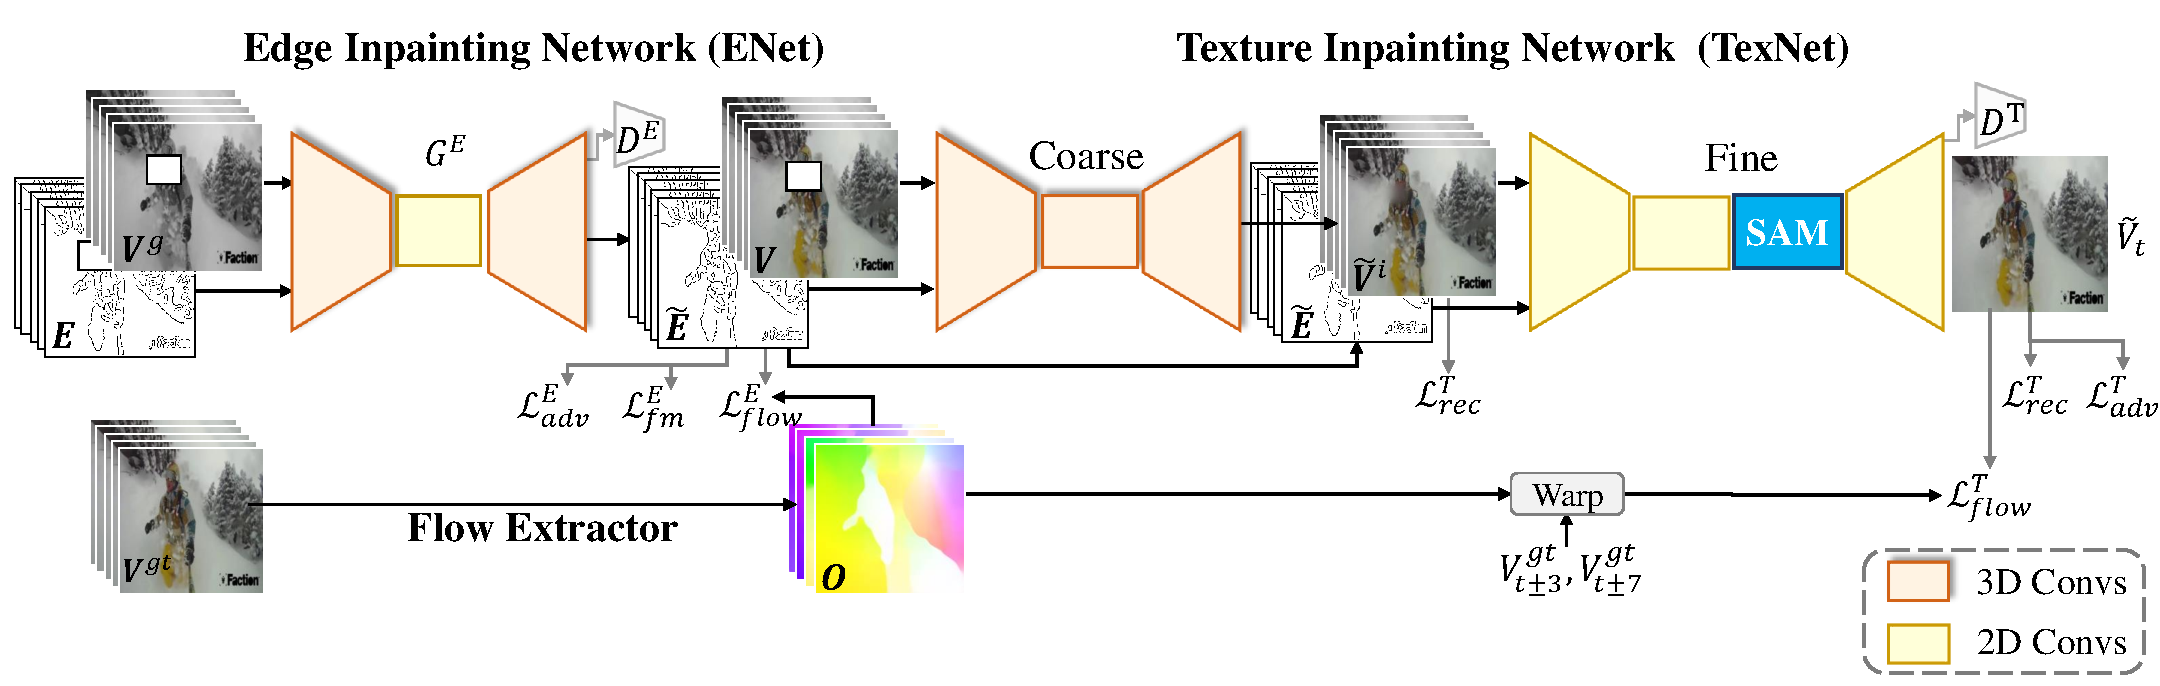
\includegraphics[width=2.05\columnwidth]{sti} % 
	\caption{The detailed architecture of our network. ENet adopts an encoder-decoder architecture to complete edges in the missing regions. TexNet utilizes a coarse-to-fine manner to inpaint the final frames. Ground truth optical flow between adjacent frames is extracted for edge consistency loss and frame warping loss. }
	%FNet is based on the backbone Resnet-101, which is associated with ENet.
	\label{fig:stiNet}
\end{figure*}

\paragraph{CNN-based Image Inpainting}
Recently, deep learning methods have achieved tremendous progress in the field
of computer vision. The tasks of image and video inpainting also have witnessed great promotion thanks to the capability of deep neural networks to capture high-level semantic information in images and videos.
%
A convolution neural network (CNN) is first introduced to directly synthesize image contents in the masked regions for image denoising and inpainting in \cite{xie2012image}.
To improve the photorealism of the synthesiszed content, a generative adversarial network is employed \cite{pathak2016context}. 
Then, Yang \emph{et al.} \cite{yang2017high} take advantages of multi-scale representation to boost details generation.
%by jointly training a generator and a discriminator in a minimax manner. 
Multiple discriminators are used to constrain both global and local coherence of image contents \cite{iizuka2017globally}.  
Yu \emph{et al.} \cite{yu2018generative} propose a contextual attention module to capture long-range information.
Subsequent approaches solve more specific problems in image inpainting, for example, inpainting irregular holes with partial convolution~\cite{liu2018partialinpainting} or employing gated convolution \cite{yu2018free} for dynamic feature selection. 
%Both these two methods want to handle image inpainting with irregular regions, which is hard for vanilla convolutions. 
%
While these methods tend to generate over-smoothed and blurry results, a two-stage approach is proposed to hallucinate edges first and then fill image colors using the edges as a prior \cite{nazeri2019edgeconnect}. 
Similarly, Xiong \emph{et al.} \cite{Xiong_2019_CVPR} predict contours of foreground objects to guide the inpainting process of masked regions.
Though high-quality static images with reasonable structure can be generated using these edge-based methods, simply extending it from image inpainting to video inpainting by 3D convolutions inevitably fails because of no guarantee on the temporal coherence, especially on the high-frequency signals. 
Besides, these methods simply utilize edges and contours as one additional channel of the image inpainting network, without exploiting a more effective mechanism to utilize the structure information more efficiently. 
In comparison, we design a structure attention module to better explore the structural guidance in synthesizing textures. 
%These image inpainting methods can obtain plausible synthesized images. 
%\cite{nazeri2019edgeconnect} introduces an edge generator to refine generated structure in image inpainting. 


%%% video inpainting 
\paragraph{Deep Video Inpainting}
%However, directly extending these state-of-the-art image inpainting methods to video domain is not an optimal solution, which will generate videos with serious temporal flickers, artifacts, and jitters. 
%Besides the challenge in maintaining temporal coherence, image inpainting methods do not fully utilize useful complementary information in neighboring frames, which could help large hole completion in videos.
Several video inpainting methods based on deep neural networks have been proposed recently, to fully utilize useful complementary information in neighboring frames.
%
The first deep-learning-based video inpainting method is CombCN \cite{wang2019video}, which jointly learns temporal structure and spatial details via 3D convolutions.
%%\cite{Xu_2019_CVPR} proposes a stacked convolution network to predict missing motion field and regards video inpainting as a pixel propagation problem. 
%
To enforce temporal coherence, features from neighboring frames are collected and refined to synthesize the missing content with recurrent feedback \cite{Kim_2019_CVPR1,Kim_2019_CVPR}. 
Instead of filling pixel colors directly using CNNs, a deep flow-guided inpainting network is proposed to estimate optical flow first in the missing region and then propagate pixel colors based on the completed flow ~\cite{Xu_2019_CVPR}.
%However, these existing methods neglect the importance of intact structure in video inpainting and typically suffer from blurs and structural cracks in the synthesized frames.  
However, these existing methods usually suffer from blurs and structural cracks in the synthesized frames since it is non-trivial to maintain fine details and sharp edges at the same time with predicting temporally coherent pixel colors. 
In comparison, we propose to explicitly complete the target structure using edges, which are efficient to predict due to their sparsity. To utilize structural information more effectively, we also introduce a structure attention mechanism. 
Under the structural guidance, more visually pleasing results could be synthesized with plausible structure and fine details. 

%Different from the methods above, we extract and refine structure information explicitly, which will generate fine-detailed video inpainting results.

%\cite{Kim_2019_CVPR} automatically removes texts in videos without mask indications, which aggregates temporal features from encoder to decoder and applies a recurrent feedback. 
%\cite{Kim_2019_CVPR1} introduces convolutional LSTM and temporal feature aggregation to obtain temporal consistency and learn information from neighboring frames. 




























